\section{Results}
\label{sec:Results}

\subsection{Magnification}
The following equation was used to calculate the magnification of the lenses:
\begin{equation}
  M = \dfrac{y'}{y}
\end{equation}
where $y'$ is the size of the image and $y$ is the size of the object. The magnification experiment compared two pictures of a line taken from the same distance. One was taken without telescope (Figure 3) and the other was taken with the telescope (Figure 4). The actual magnification can be calculated by comparing the number of pixels of both lines. The two pictures yielded 115.07 pixels without the telescope and 444.28 with the telescope, resulting in a 3.861x magnification.


\begin{figure}[!h] \label{fig:no mag}
  \begin{centering}
    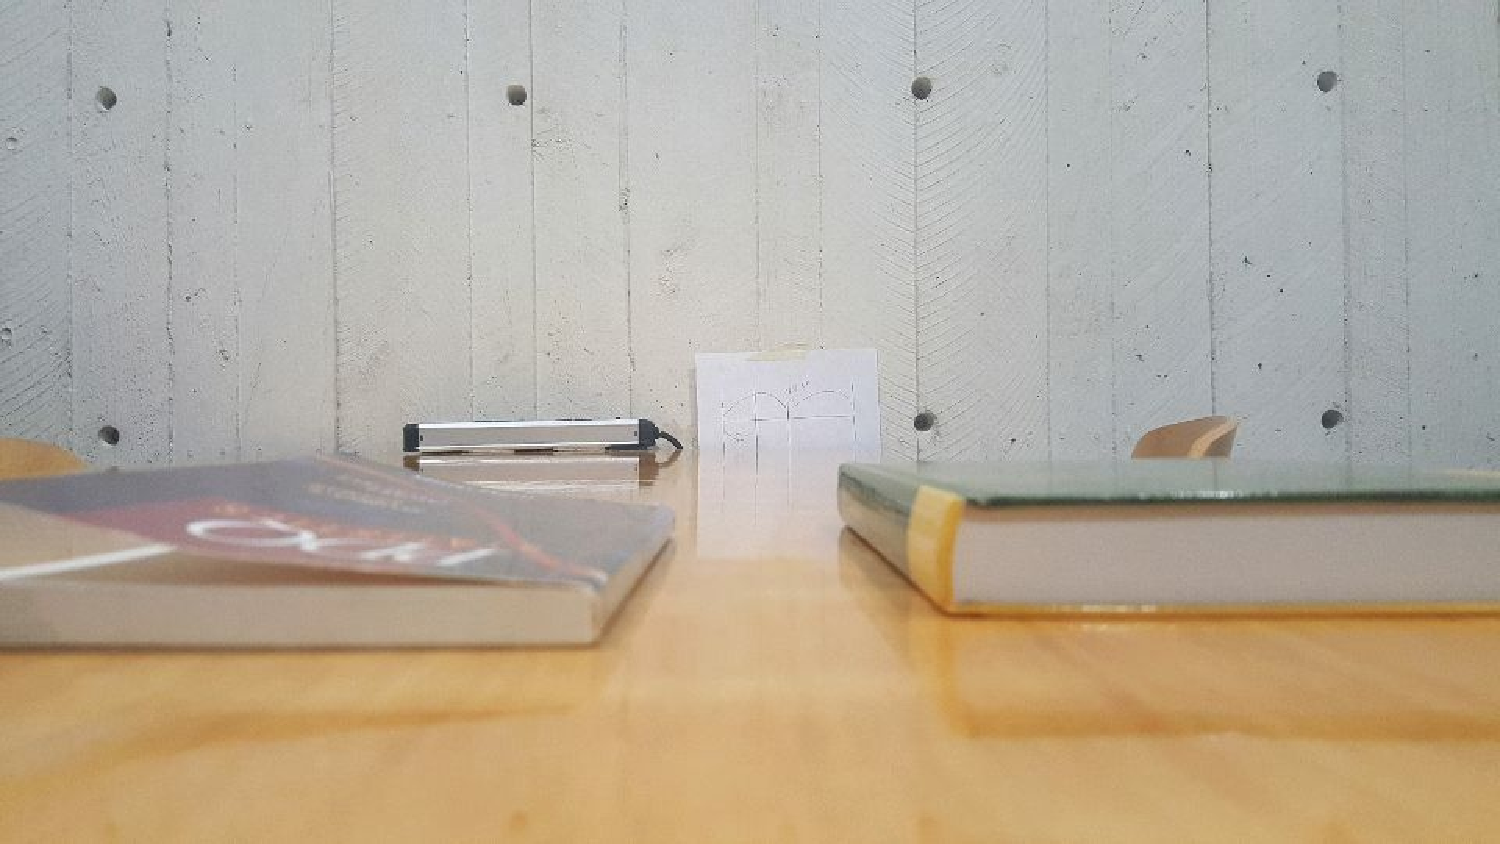
\includegraphics[width=0.45\textwidth]{./Figures/no_mag.pdf}
    \caption{Picture of object without the telescope.}
  \end{centering}
\end{figure}

\begin{figure}[!h]
  \begin{centering}
    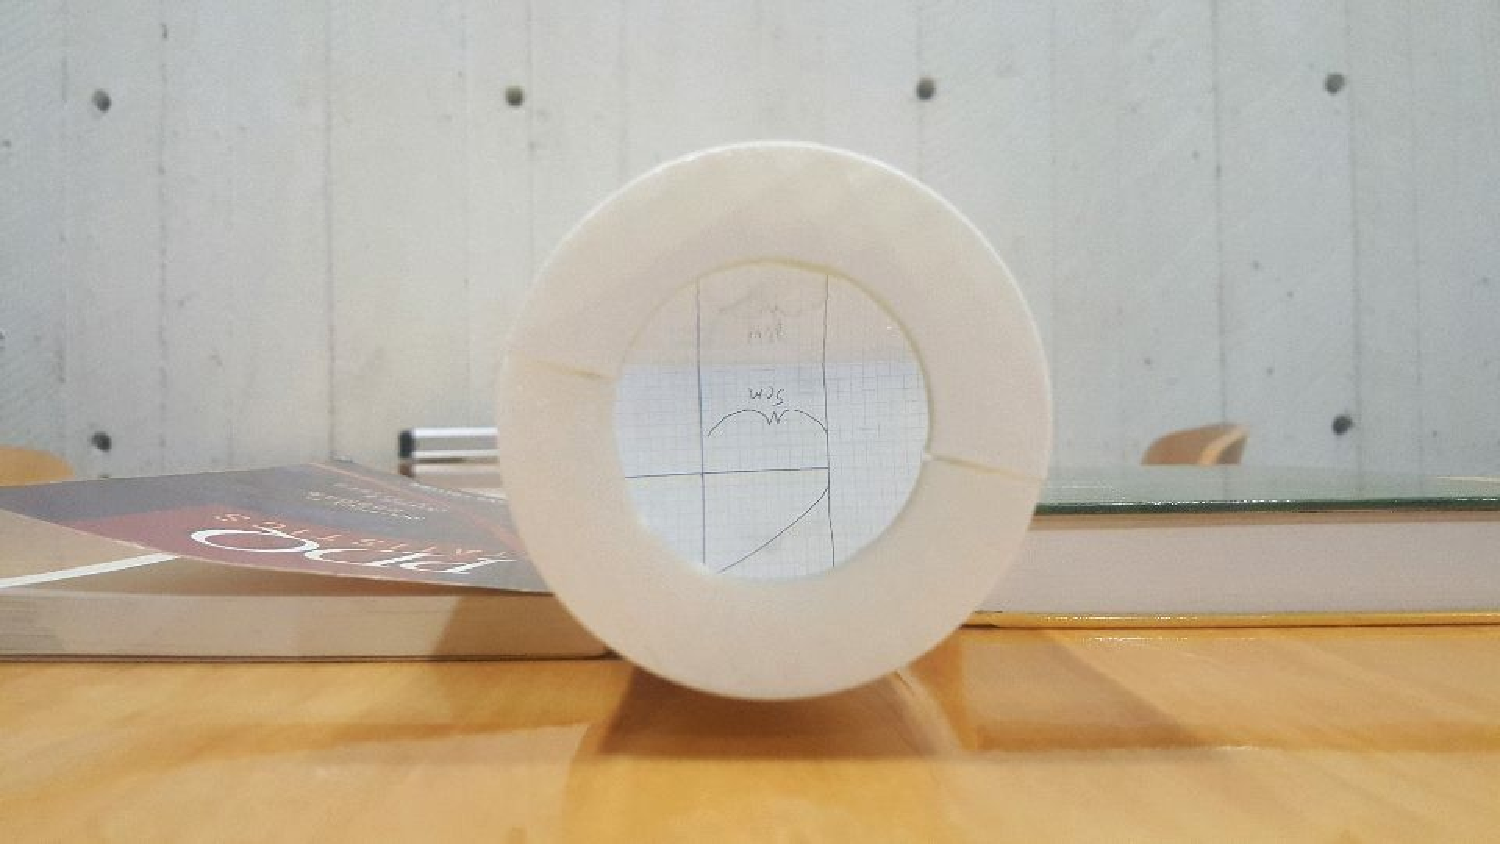
\includegraphics[width=0.45\textwidth]{./Figures/telescope_mag.pdf}
    \caption{Picture of image prodcued by the telescope.}
  \end{centering}
\end{figure}

\subsection{Cone of Vision}
\vspace*{-\baselineskip} %Removes excessive spacing

The same experiment can be used to measure the cone of vision of the telescope. The cone of vision can be calculated by measuring at what distance the \SI{5}{\centi\meter} black line on the wall begins to disappear from the range of vision. The angle $\theta$ of the field of vision can be calculated using the following formula
\begin{equation}
  \theta = 2\cdot{\taninv\left(\dfrac{r}{l}\right)}
\end{equation}
where $r$ is the radius of the cone of vision and $l$ is the height of the cone of vision (i.e. the length from the telescope lens to the screen).

\begin{figure}[!h]
  %\begin{adjustwidth}{-0.5cm}{}
  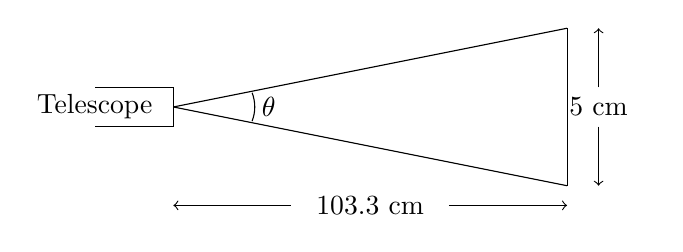
\begin{tikzpicture}[xscale = 1][yscale=1]
      \coordinate (x) at (0,0);
      \node at (x) {};
      \coordinate (y) at (7,0);
      \node at (y) {};
%      \draw[-](x) -- (y);
      %Telescope
      \coordinate (a) at (1,0.25);
      \coordinate (b) at (1,-0.25);
      \coordinate (c) at (0,0.25);
      \coordinate (d) at (0,-0.25);
      \draw[-] (a) -- (b);
      \draw[-] (a) -- (c);
      \draw[-] (b) -- (d);
      \node[] at (0,0) {Telescope};
      %Angle
      \coordinate (l) at (1,0);
      \coordinate (m) at (6,1);
      \coordinate (n) at (6,-1);
      \coordinate (theta) at (2,0);
      \draw[-] (l) -- (m);
      \draw[-] (l) -- (n);
      \draw[-] (n) -- (m);
      \pgfmathsetmacro{\lensRadius}{0.5}
      \pgfmathsetmacro{\lensHeight}{0.18}
      \pgfmathsetmacro{\startAngle}{asin(\lensHeight/\lensRadius)}
      \draw (2,\lensHeight) arc[start angle=\startAngle,delta angle=-2*\startAngle,radius=\lensRadius];
      \node[right] at (theta) {$\theta$};
      %Distance Labels
      \coordinate (g) at (1,-1.25);
      \coordinate (h) at (2.5,-1.25);
      \coordinate (i) at (4.5,-1.25);
      \coordinate (j) at (6,-1.25);
      \draw[<-] (g) -- (h);
      \node[] at (3.5,-1.25) {103.3 cm};
      \draw[->] (i) -- (j);

      \coordinate (r) at (6.4,1);
      \coordinate (s) at (6.4,0.25);
      \coordinate (t) at (6.4,-0.25);
      \coordinate (u) at (6.4,-1);
      \draw[->] (s) -- (r);
      \draw[->] (t) -- (u);
      \node[] at (6.4,0) {5 cm};
      
  \end{tikzpicture}
  %\end{adjustwidth}
  \caption{Cross section of the cone of vision.}
\end{figure}

The experiment found that the \SI{5}{\centi\meter} line begins to disappear when the telescope is \SI{103.3}{\centi\meter} away from the line. The cone of vision sweeps a full \ang{2.77}, fanning out \ang{1.39} from the center line of sight.

\subsection{Percent Error}
The percent error in the magnifcation of our telescope follows the equation
\begin{equation}\label{error}
  \%~Error = \dfrac{|M\textsubscript{theoretical} - M\textsubscript{experimental}|}{M\textsubscript{theoretical}}
\end{equation}
which produces a percent error of $43\%$. This percent error can be explained by the thin lens assumptions made by Equation 1 and Equation 2. A thin lens is a lens with a thickness much smaller than its focal length. Lens (3) has a much higher thickness to focal length ratio than lens(2), making it less ideal than lens (2). This factor most likely outweighs all other possibilities such as imperfections within the lenses and errors in experimental measurement.
